\documentclass[11pt]{article}
%% Useful packages
\usepackage[utf8]{inputenc}
\usepackage[a4paper,left=2cm,right=2cm,top=2cm,bottom=2cm]{geometry}
\usepackage{crop,graphicx,amsmath,array,color,amssymb,fancyhdr,lineno,float,booktabs,mhchem}
\usepackage{flushend,stfloats,amsthm,chngpage,times,,lipsum,lastpage,parskip,adjustbox} 
\usepackage{calc,listings,color,wrapfig,tabularx,longtable,multirow,enumitem,commath,siunitx}
\usepackage[table,xcdraw]{xcolor}
%\usepackage[numbers]{natbib}
%\usepackage[subtle]{savetrees}
\usepackage[
  nottoc
  %notlot
  %notlof
]{tocbibind}

\usepackage{hyperref}
\hypersetup{
    colorlinks=true,
    linkcolor=black,
    filecolor=teal,      
    urlcolor=teal,
    citecolor=teal,
    pdftitle={MECH0071 PSCAD Coursework},
    pdfauthor={Hasha Dar}
}

%\renewcommand\bibname{References}
\usepackage{lineno}
%%%%%%%%%%%%   Header and Footer  %%%%%%%%%%%%%
\pagestyle{fancy}
\fancypagestyle{plain}{%
  \renewcommand{\headrulewidth}{0pt}%
  \fancyhf{}%
  \addtolength{\topmargin}{-2pt}
}

\title{%
  PSCAD Coursework}
\author{Hasha Dar
}

\begin{document}
\begin{titlepage}

  \newcommand{\HRule}{\rule{\linewidth}{0.5mm}} % Defines a new command for the horizontal lines, change thickness here

  %----------------------------------------------------------------------------------------
  %	LOGO SECTION
  %----------------------------------------------------------------------------------------
  \center
  
\includegraphics[width=5cm]{Title/UCL.png}\\[1cm] % Include a department/university logo - this will require the graphicx package

  %----------------------------------------------------------------------------------------

  \center % Center everything on the page

  %----------------------------------------------------------------------------------------
  %	HEADING SECTIONS
  %----------------------------------------------------------------------------------------

  \textsc{\LARGE University College London }\\[1.5cm] % Name of your university/college
  \textsc{\Large MEng Mechanical Engineering  }\\[0.5cm] % Major heading such as course name
  \textsc{\large MECH0071 Electrical Power Systems and Electrical Propulsion }\\[1.5cm] % Minor heading such as course title

  %----------------------------------------------------------------------------------------
  %	TITLE SECTION
  %----------------------------------------------------------------------------------------
  \makeatletter
  { \huge \textsc \@title}\\[1.5cm] % Title of your document


  %----------------------------------------------------------------------------------------
  %	AUTHOR SECTION
  %----------------------------------------------------------------------------------------

  \begin{minipage}{0.4\textwidth}
    \begin{flushleft} \large
      \emph{Author:}\\
      \@author % Your name
      \\[1.2em]
      %\emph{ID No:}\\
      %0101010 \\[1.2em]
    \end{flushleft}
  \end{minipage}
  ~
  \begin{minipage}{0.4\textwidth}
    \begin{flushright} \large
      \emph{Module coordinator:} \\
      Prof. Richard Bucknall \\[1.2em] % Supervisor's Name
      %\emph{Module teaching team:} \\
      %Dr. Tim Hillel\\ % second marker's name
      %Mr. Umut Lagap
    \end{flushright}
  \end{minipage}\\[2cm]
  \makeatother

  % If you don't want a supervisor, uncomment the two lines below and remove the section above
  %\Large \emph{Author:}\\
  %John \textsc{Smith}\\[3cm] % Your name

  %----------------------------------------------------------------------------------------
  %	DATE SECTION
  %----------------------------------------------------------------------------------------

  {\large \today}\\[2cm] % Date, change the \today to a set date if you want to be precise

  \vfill % Fill the rest of the page with whitespace

\end{titlepage}

\fancyhf{}
\fancyhead[L]{MECH0071 PSCAD Coursework}
\fancyfoot[L]{Hasha Dar}
\fancyfoot[R]{ \bf\thepage\ \rm }%

\newpage
\tableofcontents
\newpage
\listoffigures
\listoftables
\newpage

\section{Question 1}
\subsection{Circuit diagram}
\begin{figure}[H]
    \centering
    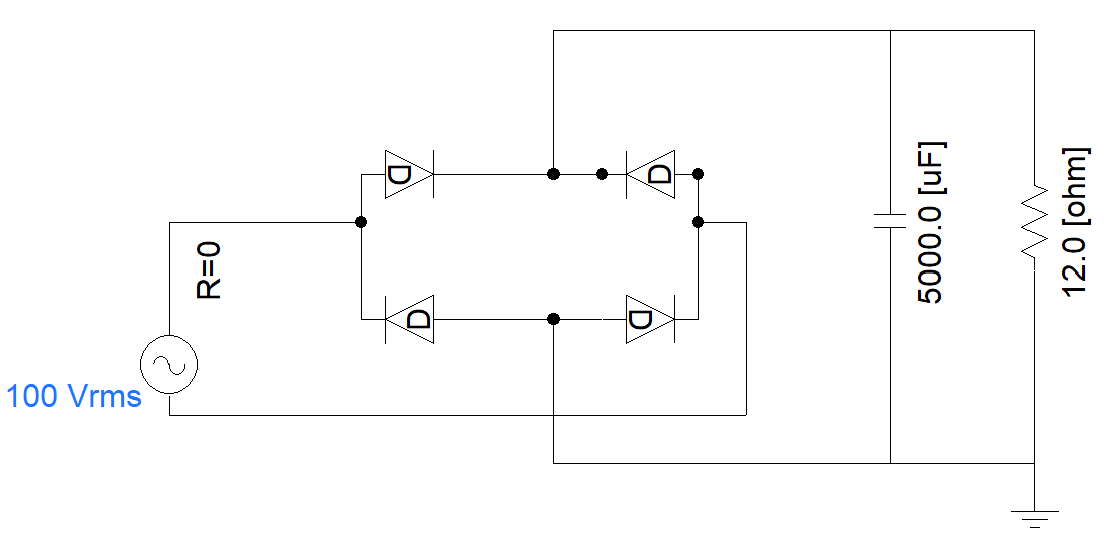
\includegraphics[width = \textwidth]{img/figure1.png}
    \caption{Circuit diagram for question 1.}
\end{figure}
\subsection{Instantaneous input voltage}
\section{Equivalent transformer}
\subsection{Circuit diagram}
\begin{figure}[H]
    \centering
    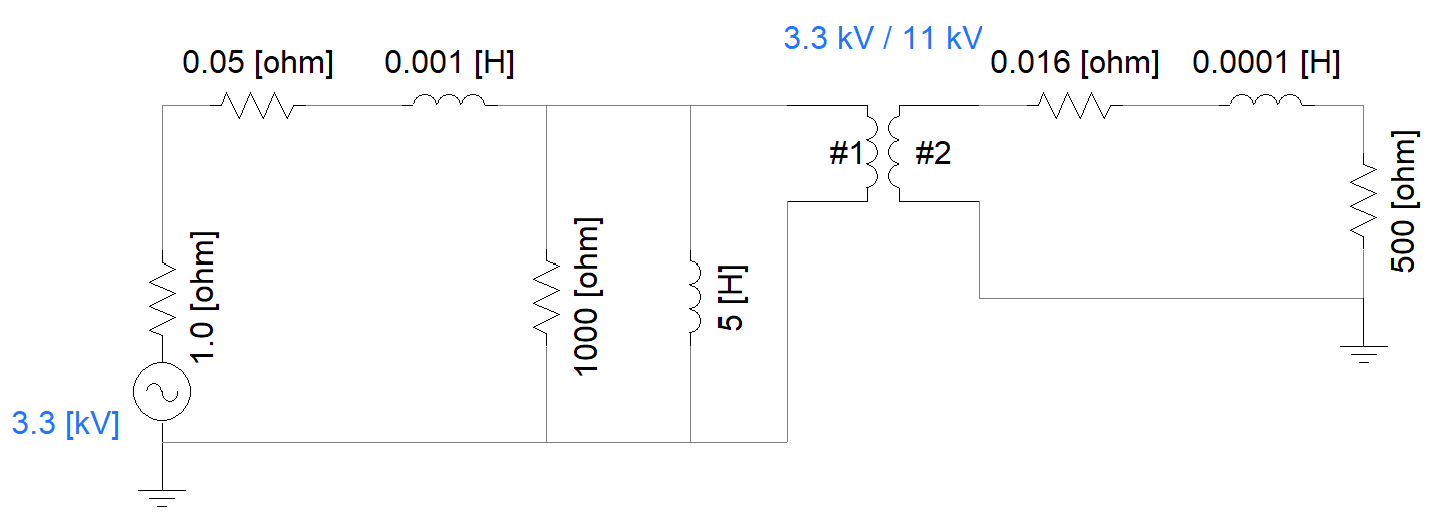
\includegraphics[width = \textwidth]{img/figure5.png}
    \caption{Circuit diagram to show equivalent transformer.}
    \label{fig:transformerCircuit}
\end{figure}
\subsection{Resistive load}
MATLAB code for this section of the assignment can be viewed in Appendix \ref{app:q2}.
\subsubsection{RMS Voltage }
The RMS voltage can be calculated using \eqref{VRMS}.
\begin{gather}\label{VRMS}
    V_{RMS} = \sqrt{\dfrac{\sum_{i=1}^n x_i^2}{n}}
\end{gather}
\begin{itemize}
    \item Simulation time: \SI{0.5}{\second}
    \item Number of data points ($n$): 2002
\end{itemize}
Using MATLAB, the RMS voltage over the time period is:
\begin{gather}
    V_{RMS,r} = \SI{10.14}{\kilo\volt}
\end{gather}
\begin{figure}[H]
    \centering
    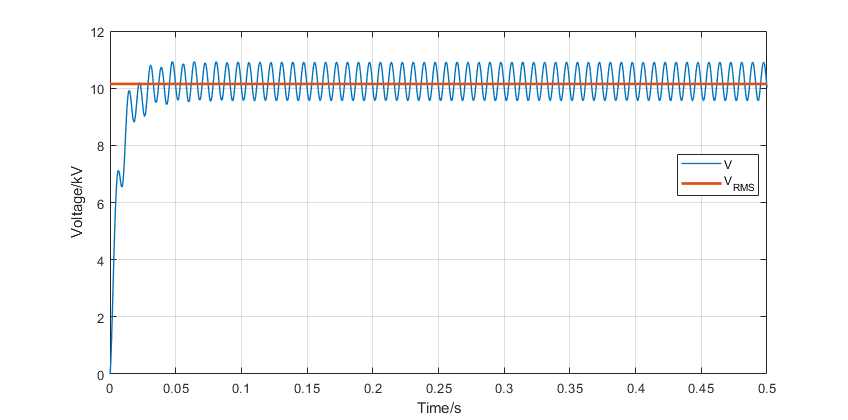
\includegraphics[width = 0.75\textwidth]{img/figure8.png}
    \caption{Voltage across load over time and value of $V_{RMS,r}$ for the time period.}
    \label{fig:VRMSResistor}
\end{figure}
\subsubsection{Power factor}
The power factor can be calculated using the following equation:
\begin{gather}
    PF = \cos \phi
\end{gather}
Using MATLAB, the converged value of the power factor was found by averaging the final values in the dataset.
\begin{gather}
    PF_{r} = 0.995
\end{gather}
\begin{figure}[H]
    \centering
    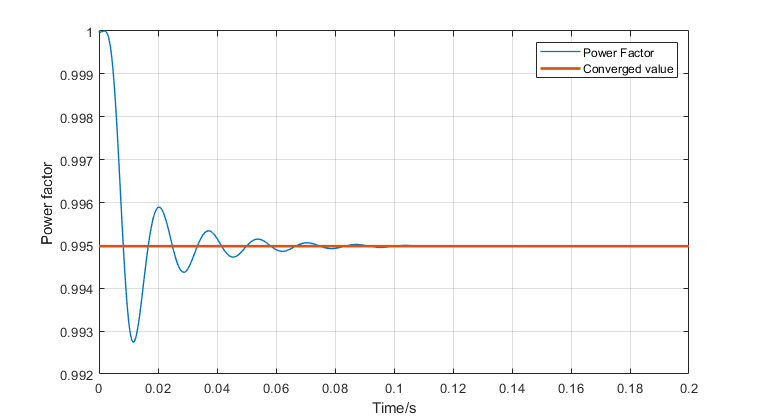
\includegraphics[width = 0.75\textwidth]{img/figure6.png}
    \caption{Power factor over time (resistor).}
    \label{fig:PFResistor}
\end{figure}
\subsection{Inductive load}
\subsubsection{RMS Voltage}
Using MATLAB, the RMS voltage over the time period is:
\begin{gather}
    V_{RMS,i} = \SI{2.79}{\kilo\volt}
\end{gather}
\begin{figure}[H]
    \centering
    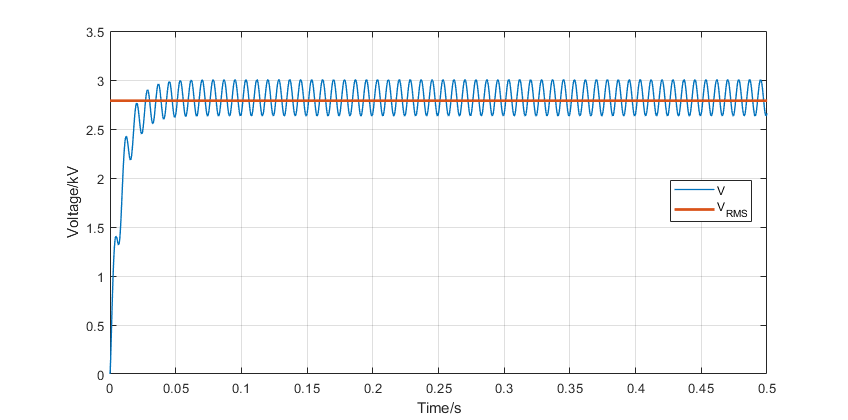
\includegraphics[width = 0.75\textwidth]{img/figure7.png}
    \caption{Voltage across load over time and value of $V_{RMS,i}$ for the time period.}
    \label{fig:VRMSInductor}
\end{figure}
\subsubsection{Power factor}
Using MATLAB:
\begin{gather}
    PF_{i} = 0.563
\end{gather}
\begin{figure}[H]
    \centering
    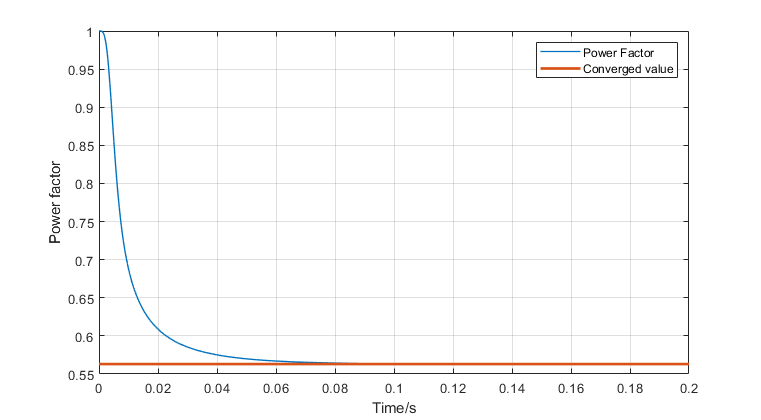
\includegraphics[width = 0.75\textwidth]{img/figure10.png}
    \caption{Power factor over time (inductor).}
    \label{fig:PFInductor}
\end{figure}
\subsection{Capacitive load}
\subsubsection{RMS Voltage}
Using MATLAB, the RMS voltage over the time period is:
\begin{gather}
    V_{RMS,c} = \SI{0.262}{\kilo\volt}
\end{gather}
\begin{figure}[H]
    \centering
    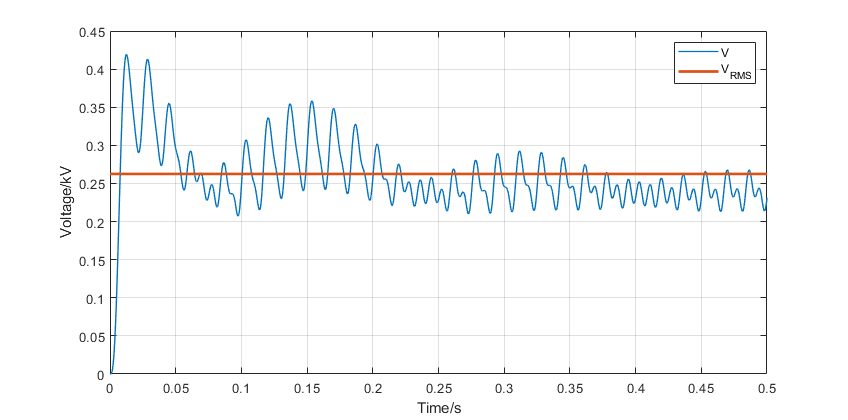
\includegraphics[width = 0.75\textwidth]{img/figure9.png}
    \caption{Voltage across load over time and value of $V_{RMS,c}$ for the time period.}
    \label{fig:VRMSCapacitor}
\end{figure}
\subsubsection{Power factor}
Using MATLAB:
\begin{gather}
    PF_{c} = -0.328
\end{gather}
\begin{figure}[H]
    \centering
    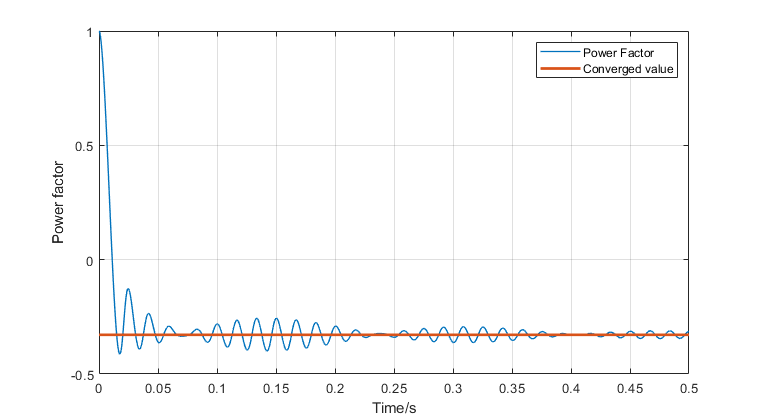
\includegraphics[width = 0.75\textwidth]{img/figure11.png}
    \caption{Power factor over time (capacitor).}
    \label{fig:PFCapacitor}
\end{figure}


%\newpage
%\bibliographystyle{unsrtnat}
%\bibliography{Refs.bib}
\newpage
\appendix
\section{MATLAB code}
\definecolor{dkgreen}{rgb}{0,0.6,0}
\definecolor{gray}{rgb}{0.5,0.5,0.5}
\definecolor{mauve}{rgb}{0.58,0,0.82}

\lstset{frame=tb,
  language=MATLAB,
  aboveskip=3mm,
  belowskip=3mm,
  showstringspaces=false,
  columns=flexible,
  basicstyle={\small\ttfamily},
  numbers=none,
  numberstyle=\tiny\color{gray},
  keywordstyle=\color{blue},
  commentstyle=\color{dkgreen},
  stringstyle=\color{mauve},
  breaklines=true,
  breakatwhitespace=true,
  tabsize=3
}
\subsection{Question 1}\label{app:q1}
\lstinputlisting[language = MATLAB]{mFiles/q1.m}
\subsection{Question 2}\label{app:q2}
\lstinputlisting[language = MATLAB]{mFiles/q2.m}
\subsection{Question 3}\label{app:q3}
\lstinputlisting[language = MATLAB]{mFiles/q3.m}
\subsection{Question 4}\label{app:q4}
\lstinputlisting[language = MATLAB]{mFiles/q4.m}

\end{document}